\chapter{Requirements}

\newpage

\section{Assignment}
\begin{figure}[H]
	\centering
	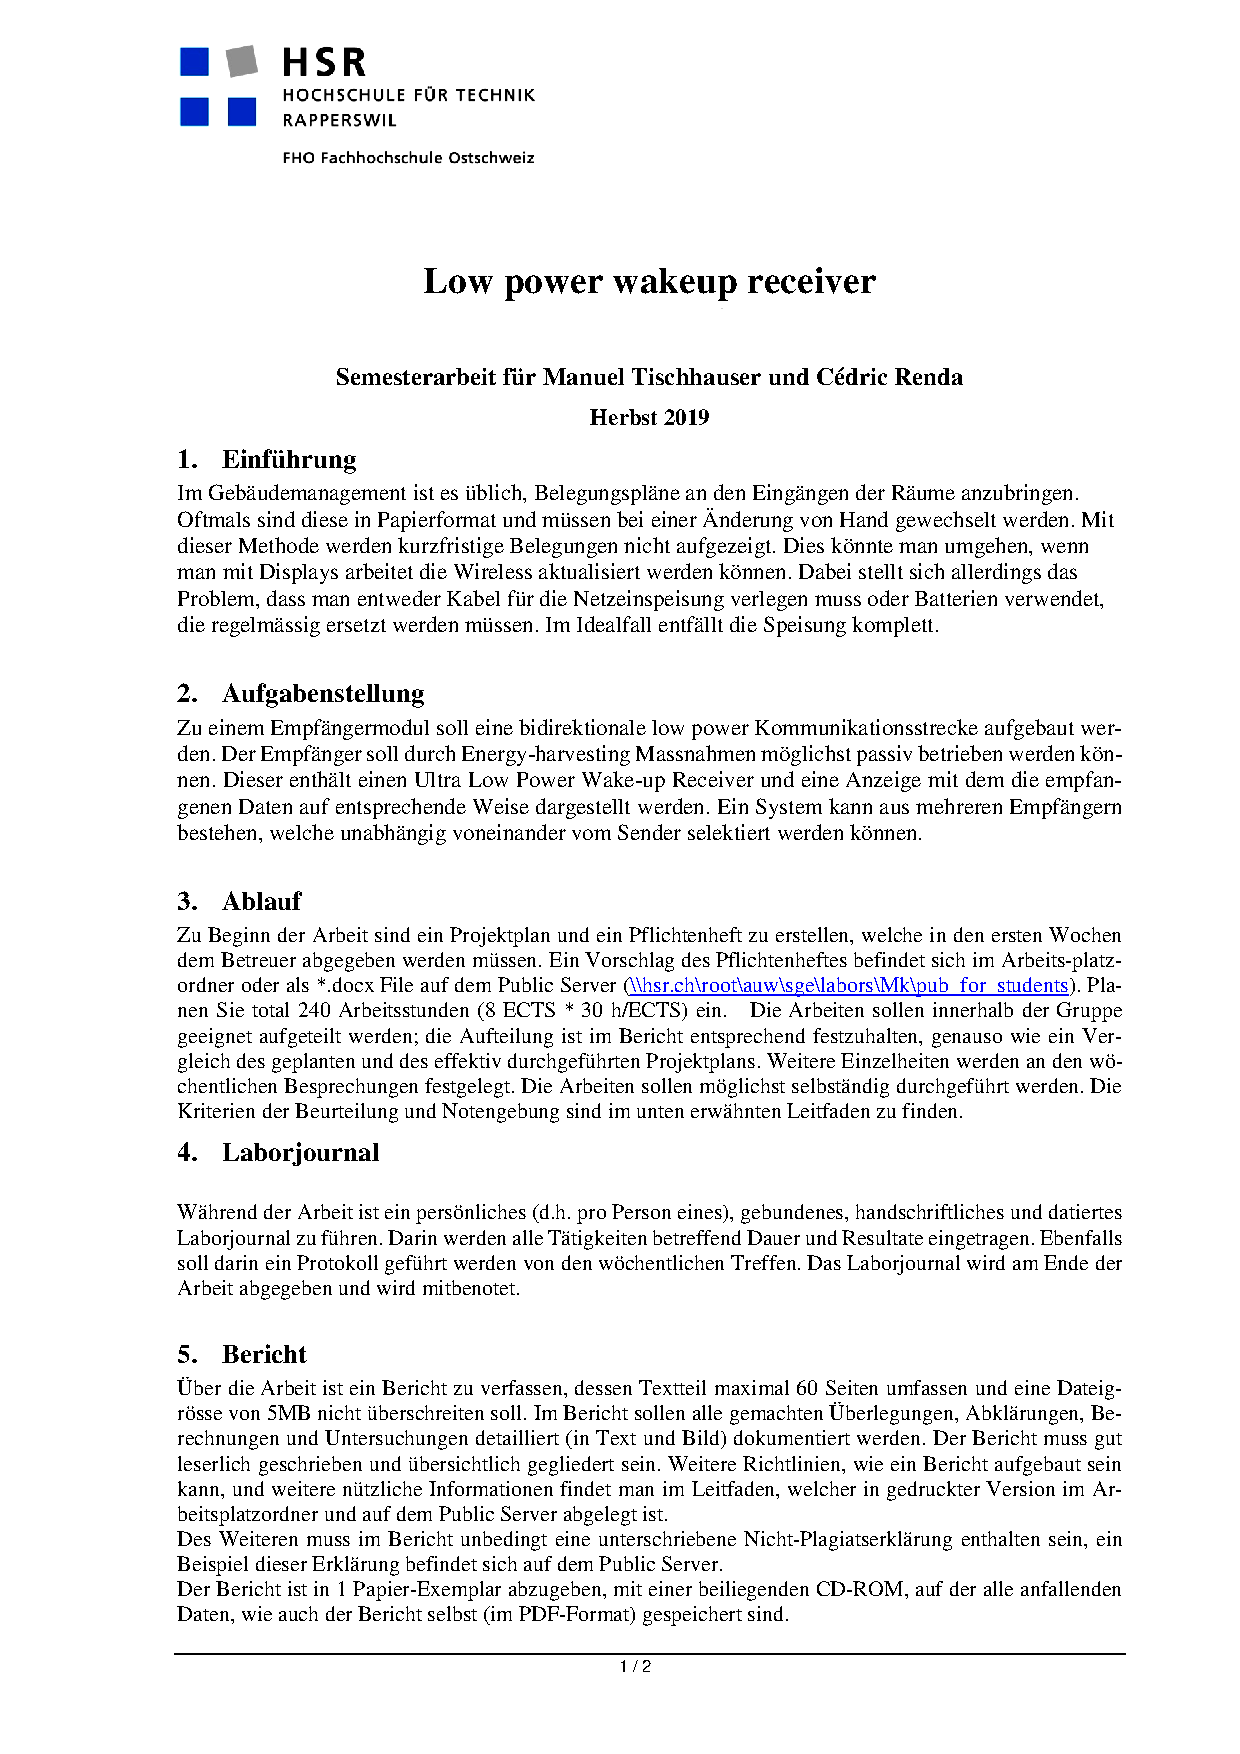
\includegraphics[trim= 0cm 0cm 0cm 0cm,page=1,width=16cm]{../Aufgabenstellung/LowPowerWakeupReiceiver.pdf}
\end{figure}
\begin{figure}[H]
	\centering
	\includegraphics[trim= 0cm 0cm 0cm 0cm,page=2,width=16cm]{../Aufgabenstellung/LowPowerWakeupReiceiver.pdf}
\end{figure}

\newpage
\section{Requirement Specification}
\begin{figure}[H]
	\centering
	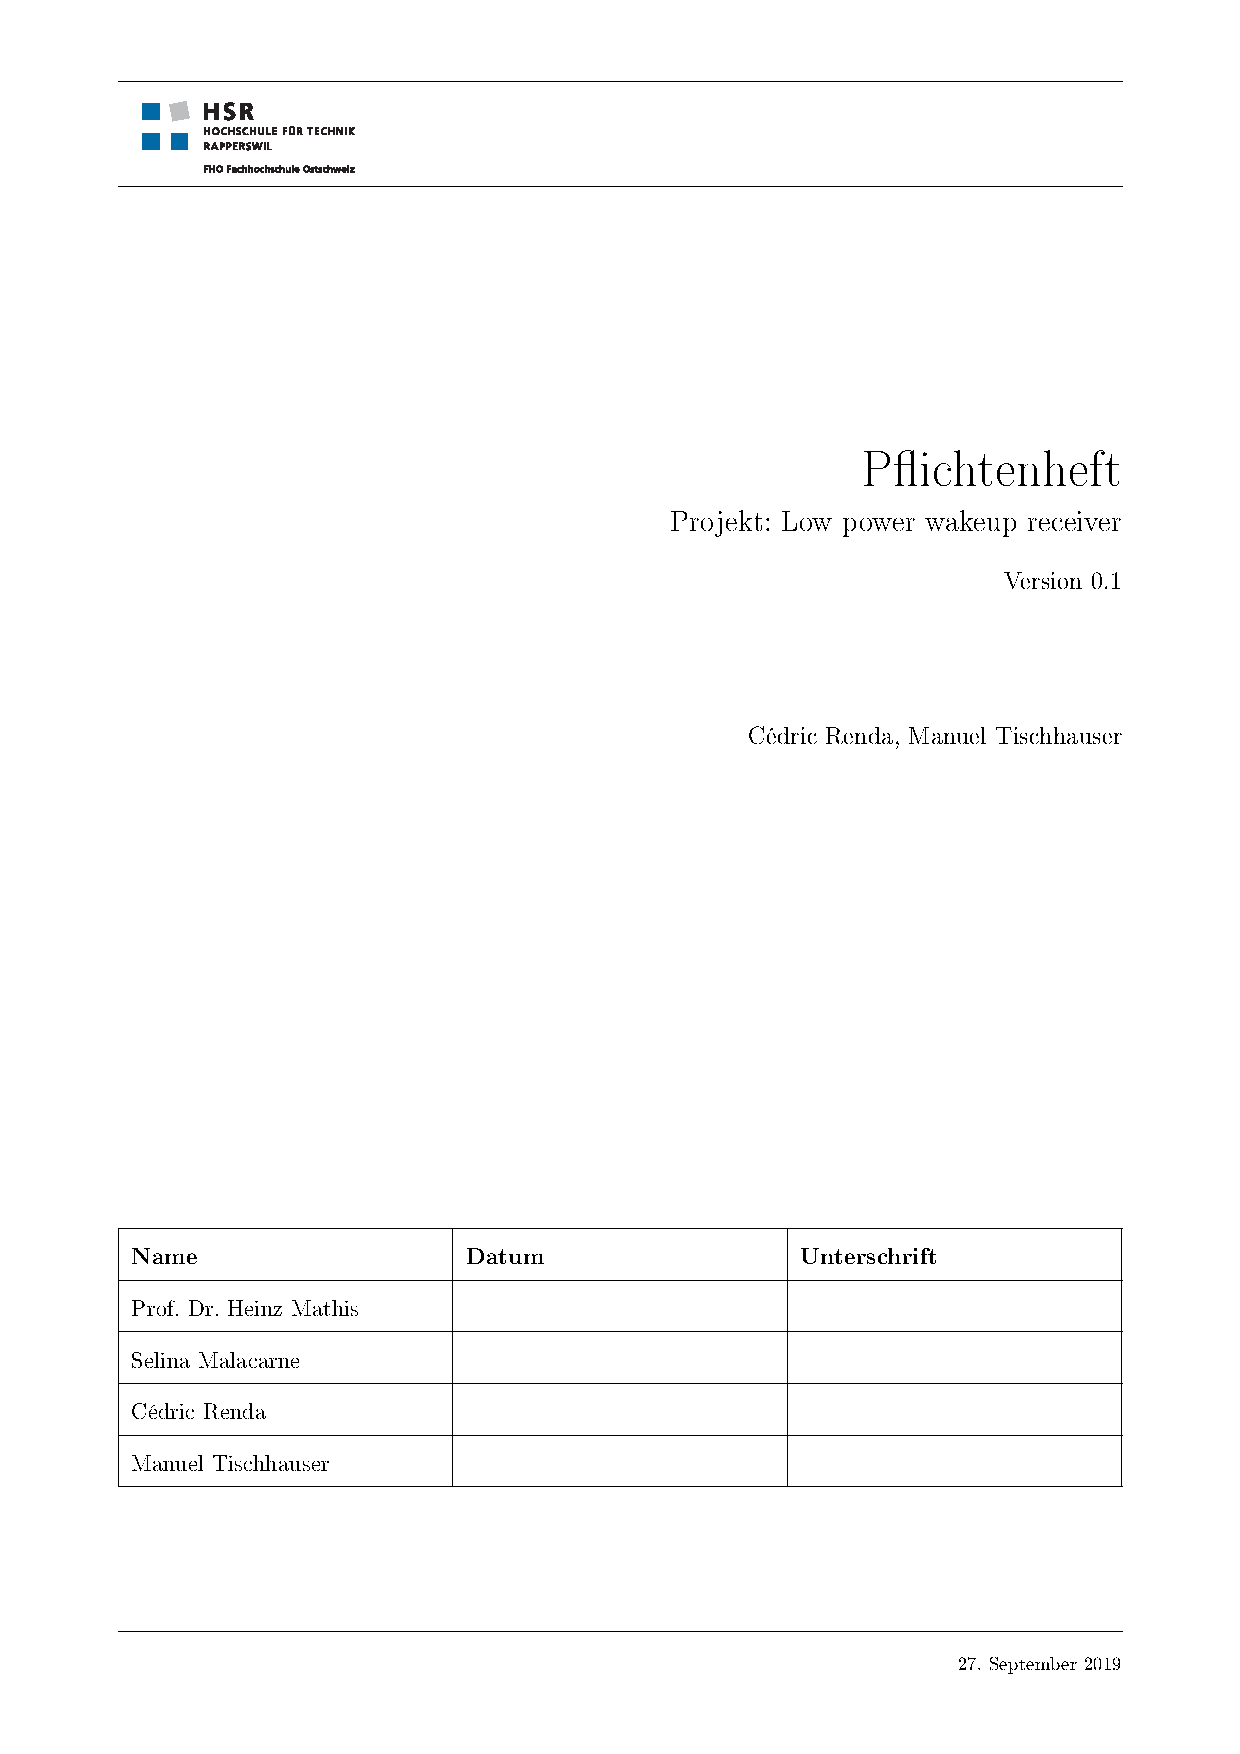
\includegraphics[trim= 0cm 0cm 0cm 0cm,page=1,width=16cm]{../Pflichtenheft/HSR_SRS_main.pdf}
\end{figure}
\begin{figure}[H]
	\centering
	\includegraphics[trim= 0cm 0cm 0cm 0cm,page=2,width=16cm]{../Pflichtenheft/HSR_SRS_main.pdf}
\end{figure}
\begin{figure}[H]
	\centering
	\includegraphics[trim= 0cm 0cm 0cm 0cm,page=3,width=16cm]{../Pflichtenheft/HSR_SRS_main.pdf}
\end{figure}
\begin{figure}[H]
	\centering
	\includegraphics[trim= 0cm 0cm 0cm 0cm,page=4,width=16cm]{../Pflichtenheft/HSR_SRS_main.pdf}
\end{figure}

\begin{landscape}
	\begin{figure}[H]
		\centering
		\includegraphics[trim= 0cm 0cm 0cm 0cm,page=5,width=22.56cm]{../Pflichtenheft/HSR_SRS_main.pdf}
	\end{figure}
\end{landscape}
